%\documentclass[fontsize=12pt, paper=a4, headinclude, twoside=false, parskip=half+, pagesize=auto, numbers=noenddot, open=right, toc=listof, toc=bibliography]{scrreprt}
\documentclass[12pt, conference]{IEEEtran}
% \documentclass[10pt,a4paper]{report}
\usepackage[utf8]{inputenc}
\usepackage[english]{babel}
\usepackage[automark]{scrpage2} % Kopf- und Fußzeilen
\usepackage{graphicx}
\ifCLASSOPTIONcompsoc
    \usepackage[caption=false, font=normalsize, labelfont=sf, textfont=sf]{subfig}
\else
\usepackage[caption=false, font=footnotesize]{subfig}
\usepackage{amsmath}
\usepackage{amsfonts}
% \usepackage{pagestyle}
\usepackage{amssymb}
\usepackage[left=2cm,right=2cm,top=2cm,bottom=2cm]{geometry}

% start new chapters on same page
\usepackage{etoolbox}
\makeatletter
\patchcmd{\chapter}{\if@openright\cleardoublepage\else\clearpage\fi}{}{}{}
\makeatother


\begin{document}
\pagestyle{empty}
\onecolumn

\clearscrheadings\clearscrplain
\begin{center}
David Steiman, 338864 \\

\vspace{8cm}

\begin{Huge}
Design, Development, and Evaluation of a blockchain-based Decentralized Access Control Protocol for Microservices \\
%Building decentralized access control list for microservices on the Ethereum blockchain.
\end{Huge}
\begin{Large}
Bachelor thesis expose \\
\end{Large}
Version 5 \\


\end{center}
\clearpage

\twocolumn
\pagestyle{useheadings}

% \tableofcontents

\section{Context}
In a microservice / federated architecture, there are different demands on security. The focus of today's microservice sources is mostly for the question: how to ensure that at request time all information needed for access decisions is available for processing. In details, the topics cover authentication (e.g., OpenID, IAM, SAML) to identify the requesting subject and authorization (e.g., OAuth 2, JWT) to gather all information about the authorization of the subject. The next question is about, how to make a decision. For this purpose, there are different approaches to access control enforcement, like role-based access control (RBAC) or attribute-based access control (ABAC). These concepts are simple, but lack on expressibility in complex access control requirements.  For fine-grained access control, a well-established way is using ``access control lists`` (ACL) for a detailed definition of policies, which often occur in monolithic applications. While tools like JWT make it unnecessary to store a state of a session, ACLs have to be persisted in a way accessible to all microservices. Moreover, someone has to manage the ACL configuration. In particular, in federated systems, where services belong to a certain party, every member has to trust this policy administrator.
Consequently, the core idea of ACLs lacks in two points: decentralization and trust.


The DACL concept relies on the model of domain-based distributed systems. In favor of this idea, domain is described as ``the realm of knowledge [..] of the software system being designed`` \cite{b2} which ``can be used to group
objects in a hierarchical structure, to apply a common security policy [..] of large distributed systems.`` \cite{b1} Based on the concept of Yialelis, which is close to a system this thesis aims for, access control is designed with ACLs. An entry of the list contains the requesting subject, requested target and access rules defined for those. A reference monitor enforces policies. Although his idea has a focus on distributed systems, the concept assumes the presence of a policy administrator, which is performing the overall security configuration. So this access control mechanism requires trust in a central authority. \\

\begin{figure}[!h]
  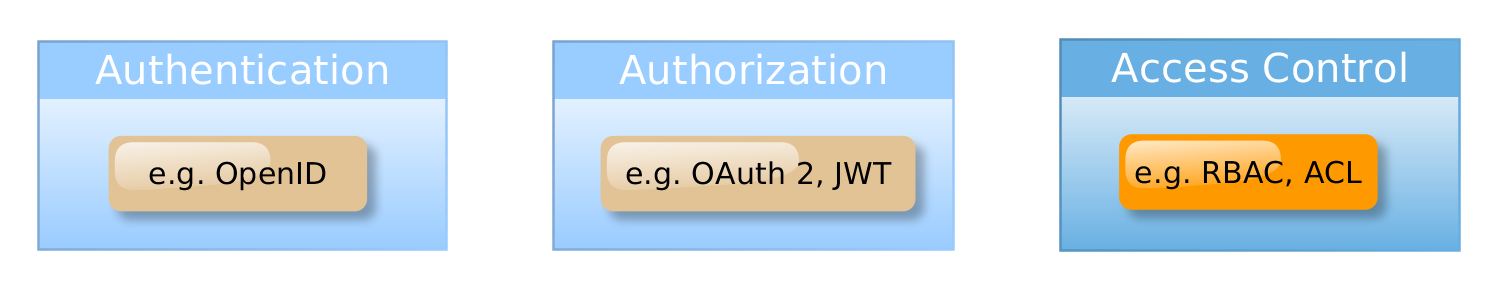
\includegraphics[width=\linewidth]{figures/access-control.png}
  \caption{DACL for access control in microservices.}
  \label{fig:access-control}
\end{figure}

This thesis introduces a ``decentralized access control list`` (DACL) protocol. Assuming the presence of an identity management and authentication, DACL describes how to enforce authorization policies, being fully decentral and eliminating the need for a central authority (trustlessness). 

In favor of decentralization, DACL requires the underlying persistence be managed in a distributed manner, and that stored data cannot be changed later. For trustlessness, DACL supposes a smart contract is coordinating all state-changing operations.

In favor of decentralized governance of microservices, the protocol itself does not cover technical details, to leave the implementation open to the service. The mechanism will be applied to an exemplary scenario to show, how these protocols should be used and implemented using Ethereum and IPFS.


\section{Example scenario}

\begin{figure}[!h]
\centering
  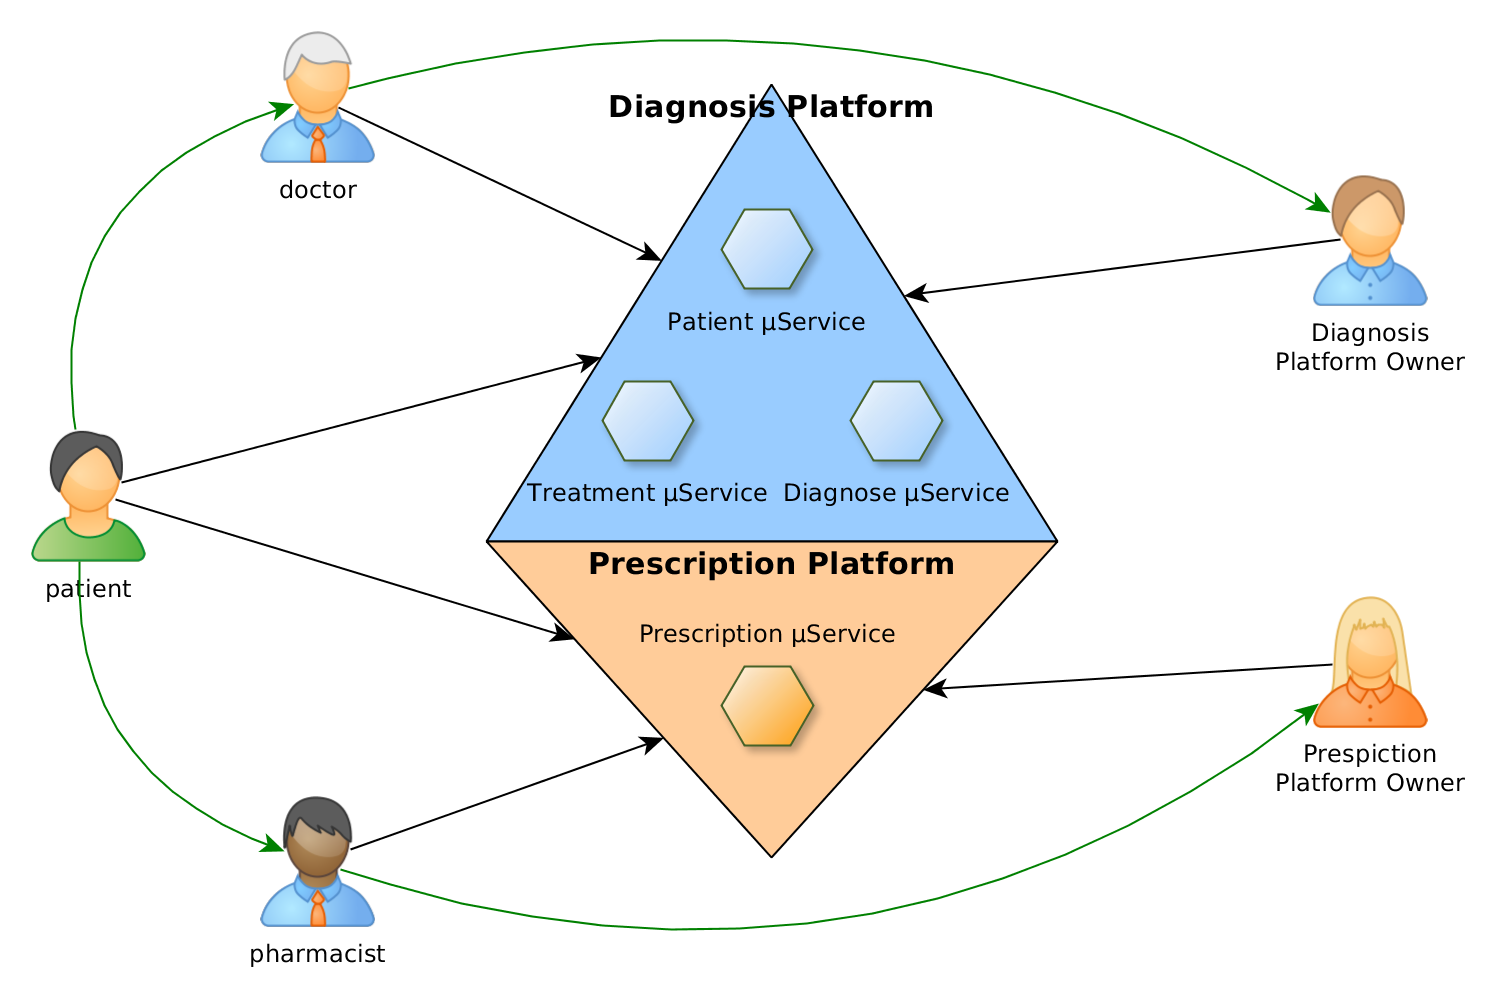
\includegraphics[width=\linewidth]{figures/platform.png}
  \caption{architecture of an eHealth Platform.}
  \label{fig:platform}
\end{figure}

The scenario describes a federated eHealth application platform for diagnoses and prescriptions. During treatment, a doctor declares several diagnoses and prescribes prescriptions for his patients. In this scenario, two parties are maintaining the eHealth platform, which consists of a diagnosis and a prescription platform. As medical data of a patient is highly sensitive, the access control policies are complex. On the one side, the patient should always be able to supervise the permission on his data, but allow exceptions for his doctor, e.g., to open access to diagnoses to collaborating doctors. On the other side, both doctors and pharmacists might become patients as well, so approaches like RBAC do not fit well. The green arrows in figure \ref{fig:platform} show the permission grant direction, while the black arrows show the common requests done by the different users. As data relating to a user should only be under the user's control, maintaining a central policy authority is not acceptable. Using centralized ACL mechanism also means, one node (or a centrally managed group of nodes) is responsible for storing the policies and allows this central authority to bypass the policies and manipulate the data.

The thesis claims to show, how DACL helps to construct a decentralized access control mechanism, to ensure patients keep control over their data by implicitly changing the security policies of the eHealth platform.

\section{Problems}



\subsection{Trustlessness}

The first core problem of DACL is trustlessness. Trustlessness means, no one has special privileges over the state of the policies.  In other words: there is no need to trust someone. So the subsequent problems here are: \\

\subsubsection{Network members and proposal handling}

The DACL smart contract allows a set of participants (e.g., Ethereum wallets) to be part of a network, where every member is permitted to interact with the smart contract. As there is no network administrator, the protocol must define how new members can join or how to remove malicious participants. 

As there is no central policy authority as well, which can perform changes on its behalf, the protocol must define a proposal handling for changes. The basic idea says every participant can read the policies, propose changes and vote on them. By default, all participants are forced to vote on any proposal. However, there are use-cases, where a participant is not required to participate in the voting process for some reason. The protocol must define the proper conditions when change proposals are accepted.

In the case when multiple policy change proposals are pending the network must end up in a state, where all valid policy change proposals are checked in.

\subsubsection{Access policy enforcement}

Comparing to the reference monitor from Yialelis' domain security model, the DACL protocol should define, how policies are enforced. Assuming technical requirements violates the microservice approach of decentralized governance the protocol should specify, how the policies are applied. Optionally it could be discussed, how other members can prove the policy enforcement.

\subsubsection{After-the-fact mandate changes}

Although only participants known by the smart contract are permitted to interact with the policies, there still are business use-cases to make exceptions on these mandates. To cover similar exceptions on a ``consortium blockchain``, the Hyperledger requirements work group released a set of 8 requirements \cite{a1}, where the following are relevant to the DACL design:

\begin{itemize}
\item{a member(anchor) shall be able to sign over its authorization to another member (guardian) after the fact. This requirement accords to the following two scenarios:
    \begin{itemize}    
    \item     {anchor loses its authorization}
    \item {anchor maintains its authorization over the smart contract}
    \end{itemize}
}
\item the network shall be able (e.g., via a blockchain consortium) to sign over the authorization over a smart contract from anchor to another member
\item it should be possible to re-assign the authorization
\item all assignments shall not require handling over private keys
\end{itemize}

As the DACL does not define a consortium, the other requirements do not fit well here.

\subsubsection{Policy storage}

Agnostic to the storage design, the owner of a node should not be able to change the data. Manipulating the value of the stored data should make the data invalid.


\subsection{Decentralization}

The second problem of DACL is about reducing the responsibility of a single participant and coordinating all tasks around communication and persistence completely in a distributed manner. In particular:

\subsubsection{Costs of operation}

Putting data on the blockchain is expensive, so it must be clarified, which part of the data is ``on-chain`` and which ``off-chain``. In particular, how to refer to the off-chain-stored data. 

Considering the core component of DACL is an Ethereum smart contract, every writing operation costs some fees in Ether (the Ethereum cryptocurrency) to be paid by a participant. Also, the complexity of the contracts final implementation is relevant for the running costs, as these depend on the number of instructions processed in Ethereum. When a participant runs out of gas, he becomes unable to communicate with the network, so the contract must regulate this costs with methods like auto-refilling and define how the network responds to frozen participants. For example, implementing a health check, where every participant writes the current timestamp on the blockchain can prevent this block on proposals, but increase the running costs.

\subsubsection{Performance}

The performance of DACL can be narrowed down to the response time for a request, which involves an access decision, and the duration for new proposals getting committed and propagated to all participants. The entire state can be stored in a single document, containing the full policy configuration. Consequently, a proposal consists of a whole state, too. Handling these policies unstructured may heavily affect the time a participant needs to iterate over the proposal. In a different approach a proposal consists only of a set of changes, so the current state is the result of all accepted changed applied after each other. Without caching, accumulating the changes may cause many requests, what affects the response time.

\subsubsection{Policy storage}

No node should form a single point of failure. As of the CAP theorem, there is no way to guarantee consistency, availability, and partition. An access control decision must be possible at any time. There should be a tradeoff between consistency (ensure new policies are always available right after their commit), or partition (avoid storing a complete policy configuration state on every node).

\subsubsection{Horizontal scalability of the microservices}

Microservices are often designed according to the twelve-factor app specification \cite{site1}. Processes and Disposability are the key factors for horizontal scalability, as microservices run replicated and might be terminated at any time. Considering DACL is causing a time-intensive overhead for building a valid state, this would harm these two factors and consequently impact the horizontal scaling abilities of DACL secured microservices. A vivid example would be if every microservice must first synchronize with the entire Ethereum blockchain from scratch, what would take hours for a new replica to be running.



\section{Proposed solution approach}


\begin{figure}[!h]
    \centering
  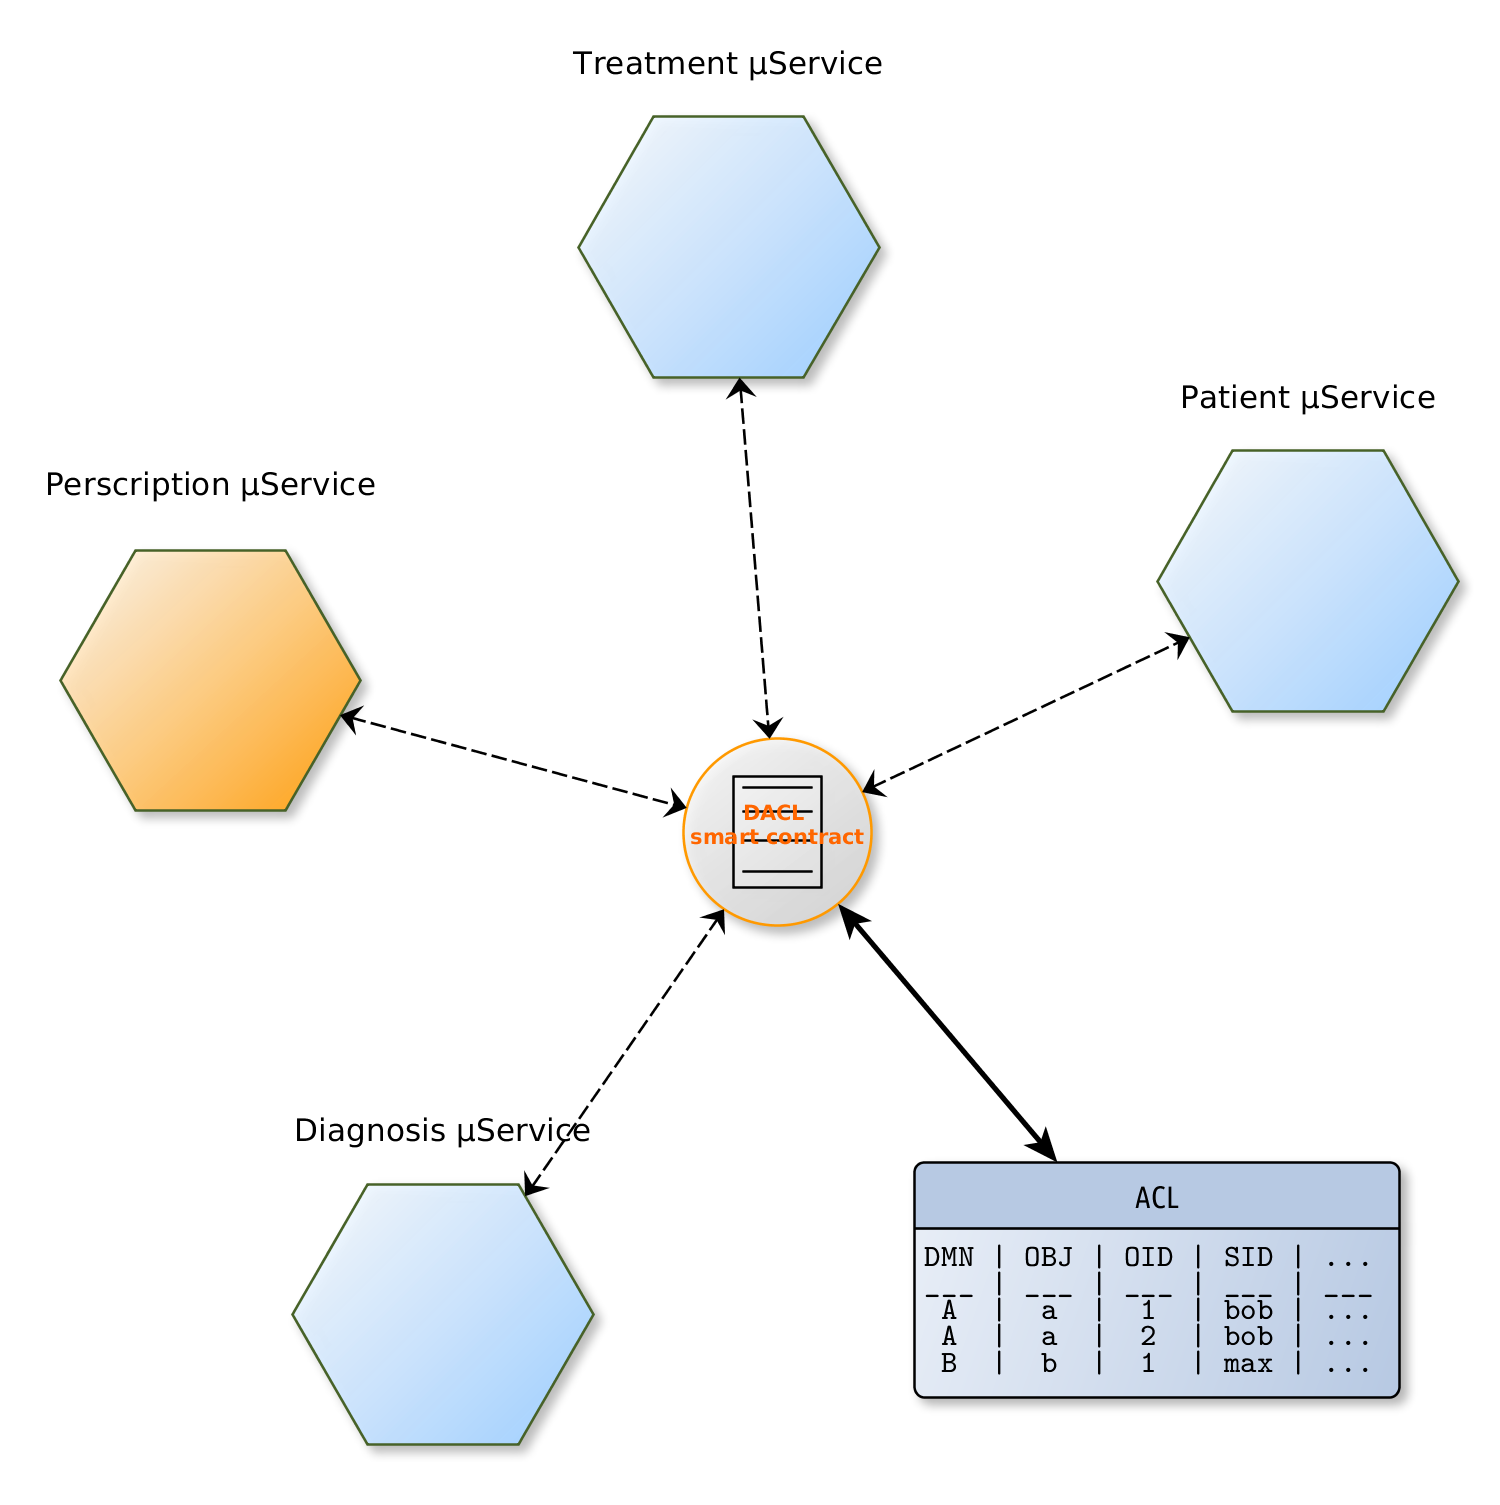
\includegraphics[width=\linewidth]{figures/DACL-basic.png}
  \caption{Basic DACL architecture applied to scenario.}
  \label{fig:basic-dacl}
\end{figure}

The proposed distributed access control list protocol (DACL) claims to give a solution to the problems. At the core, all members of the DACL defined network interact with a single smart contract, which provides the actual state of the ACL and coordinates changes to this state. 

\newpage

\subsection{the DACL protocols}

DACL is designed using the following sub-protocols:

\subsubsection{access decision protocol}

The protocol first defines an access control entity $ ace \in \mathbb{ACL} $, which is in an access control list $ \mathbb{ACL} $, defined by:
\begin{footnotesize}
$
\mathbb{ACL} = \{ (domain, oid, uid, sid, permission, order) : domain, oid, uid, sid \in \Sigma^*,  permission \in \{0,1\}^4, order \in \mathbb{N} \} 
 $
 with: \\
 $ domain = $ the domain that owns the object  \\
 $ oid = $ the object identifier of target object \\
 $ uid = $ the objects unique identifier \\
 $ sid = $ the unique identifier of the requesting subject \\
 $ permission = $ 4 bits for create, read, update and delete permission \\
 $ order = $ the order of this entry in a set of matched rows \\
 \\
\end{footnotesize}
This infinite discrete set can be represented as the following table:

\begin{table}[!h]
\centering
\tiny
\begin{tabular}{|c|c|c|c|c|c|}
\hline \rule[-2ex]{0pt}{5.5ex} domain & OID & UID & SID & permission & order \\ 
\hline
... & ... & ... & ... & ... & ... \\
diagnoses & diagnosis & 123 & Alan & 0111 & 1 \\ 
diagnoses & diagnosis & 123 & Dr. Bob & 0111 & 2 \\ 
diagnoses & diagnosis & 123 & @any & 0000 & 3 \\ 
prescriptions & prescription. & 234 & Alan & 0100 & 1 \\ 
prescriptions & prescription & 234 & Pharmacist & 0100 & 2 \\
prescriptions & prescription & 234 & Dr. Bob & 0111 & 3 \\
prescriptions & prescription & 234 & Dr. Colin & 0111 & 4 \\
... & ... & ... & ... & ... & ... \\
\hline
\end{tabular}

\end{table}


Every microservice acts as a participant for a domain (by owning a private key known to the smart contract). 

To evaluate this ACL for a given object and subject, a participant iterates over all access control entries for its matching domain in the defined order. The first match is providing the decision if access is granted. A participant is free to use any convention for identifying a single subject, a group of users or a role. 


\subsubsection{policy coordination protocol}

The policy coordination protocol describes how exactly parties can change the ACL. Given the fact, all communication is done via the DACL smart contract, figure \ref{fig:proposal-handling} describes how a successful reconciliation should proceed. 

\begin{figure}[!h]
\centering
\subfloat[initial state]{
    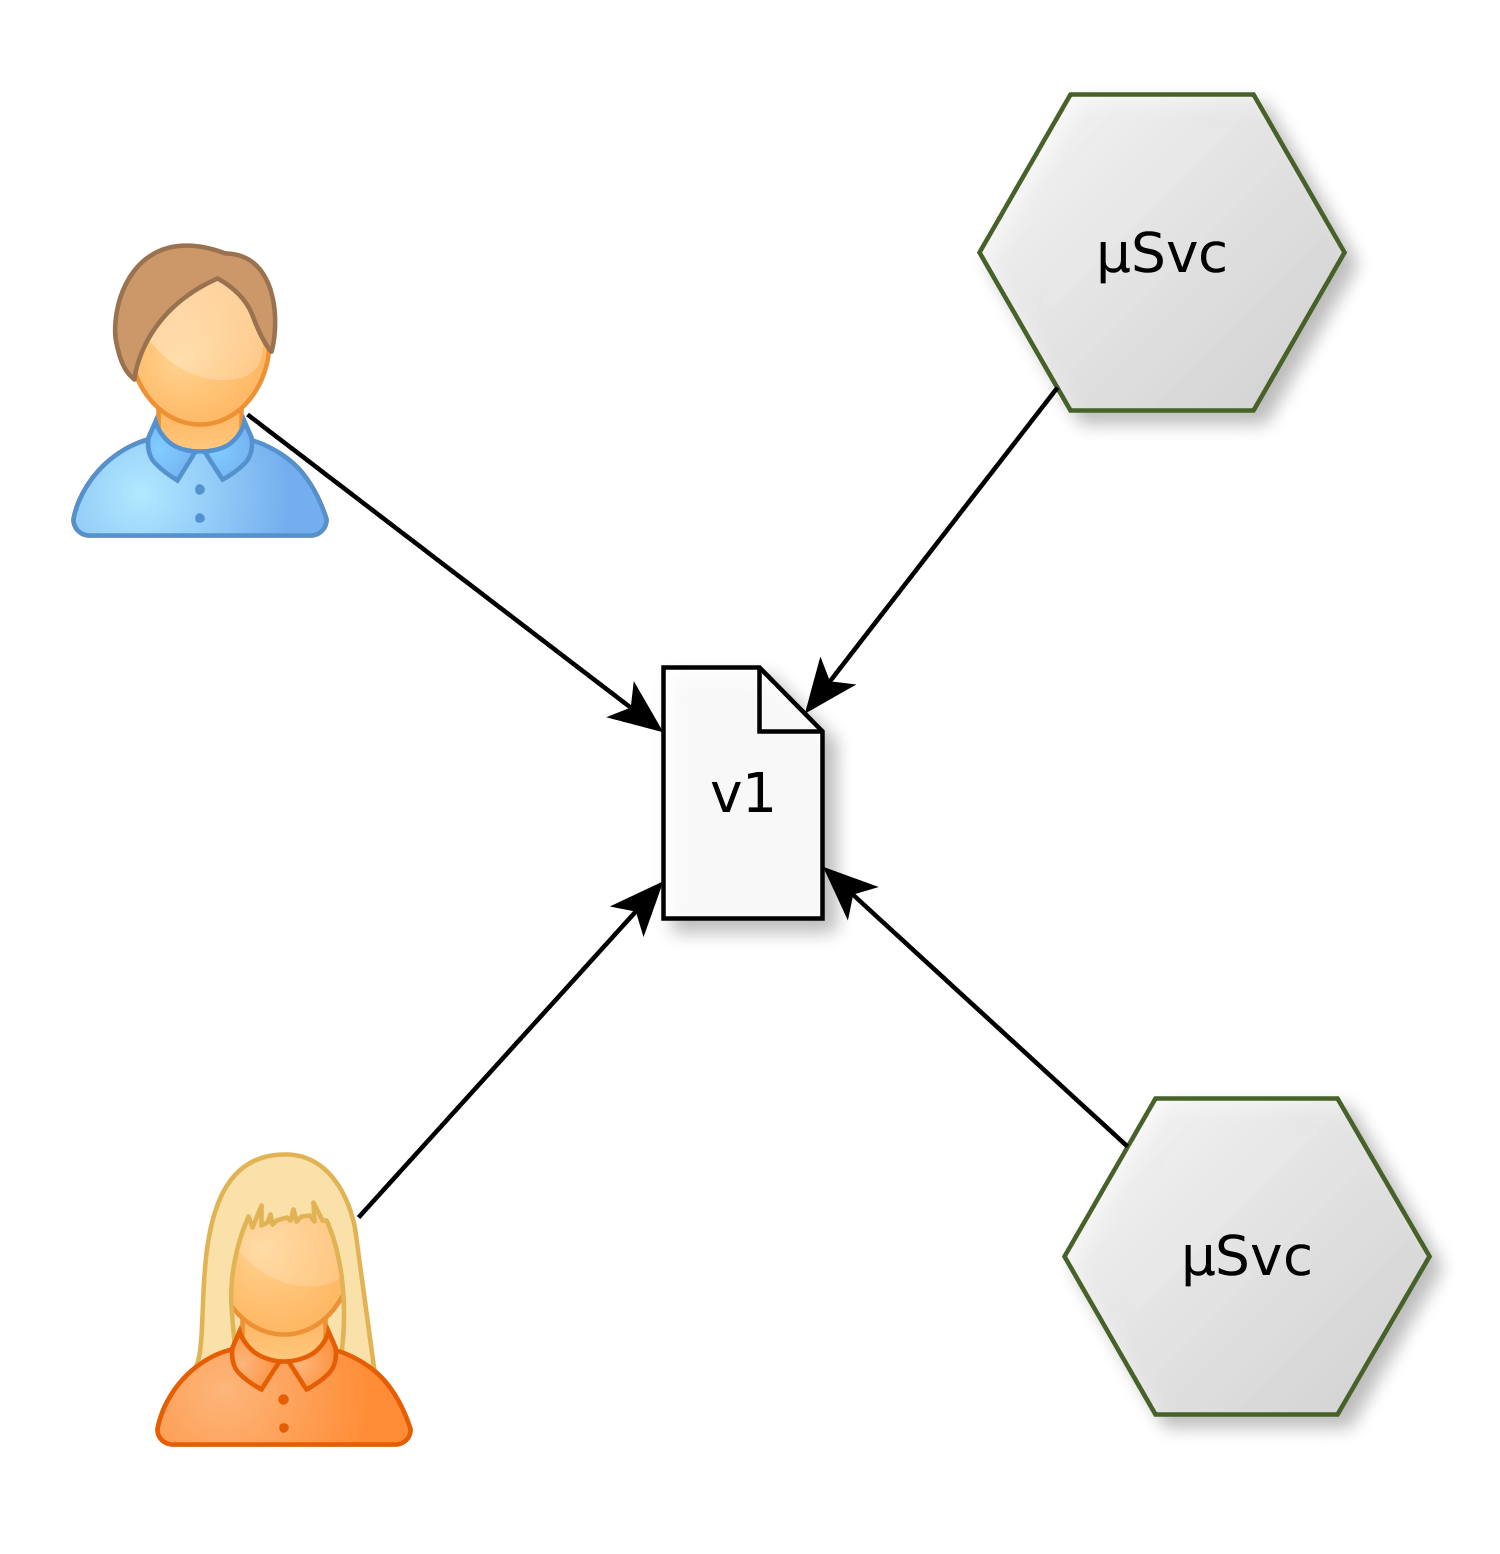
\includegraphics[width=0.32\linewidth]{figures/ACP-initial.png}
} \hfill
\subfloat[state change proposal]{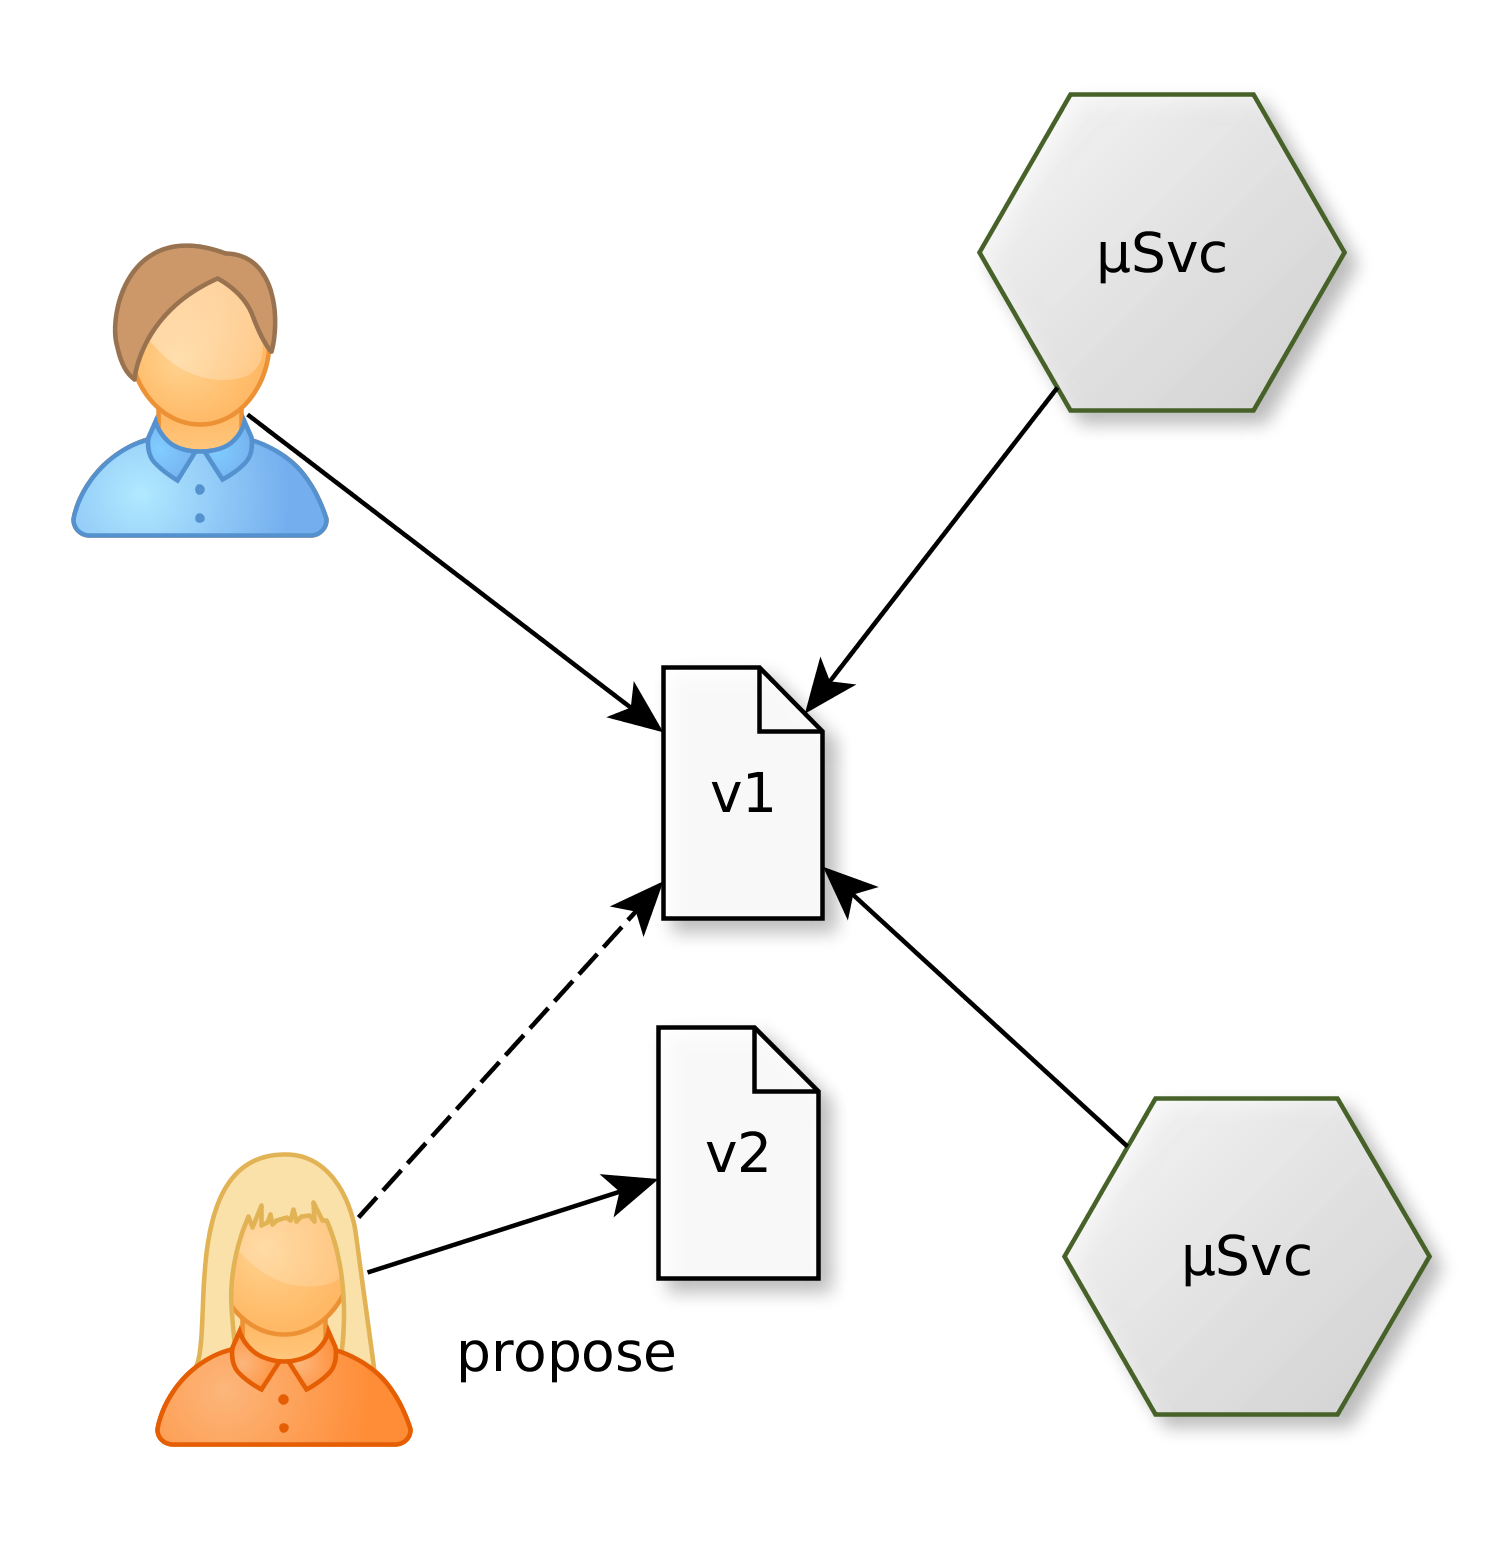
\includegraphics[width=0.32\linewidth]{figures/ACL-propose}} \hfill
\subfloat[accepting new policy]{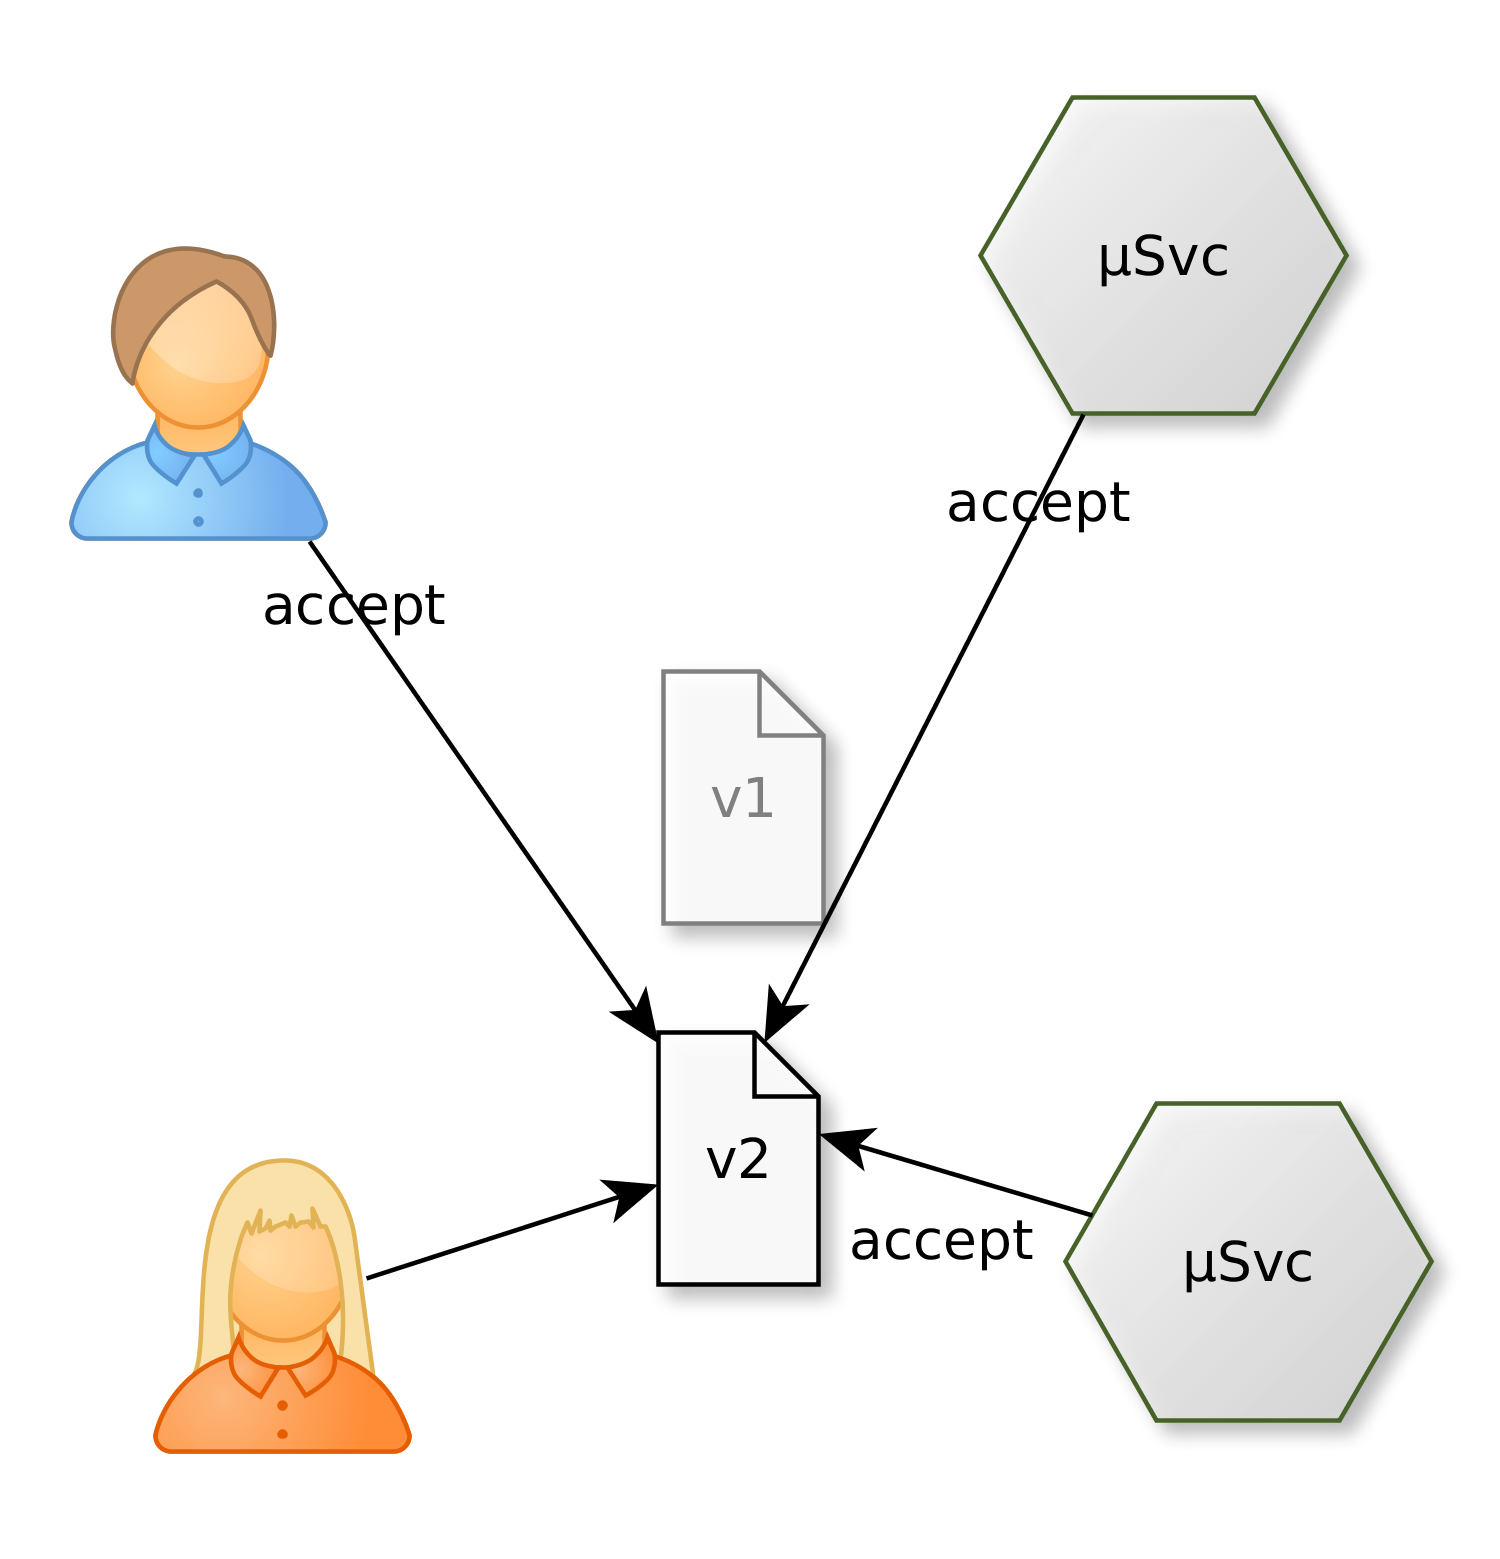
\includegraphics[width=0.32\linewidth]{figures/ACP-accept.png}} \\
\caption{example of successful change proposal}
\label{fig:proposal-handling}
\end{figure}


%\begin{figure}[!h]
%\minipage{0.32\textwidth}
%
%  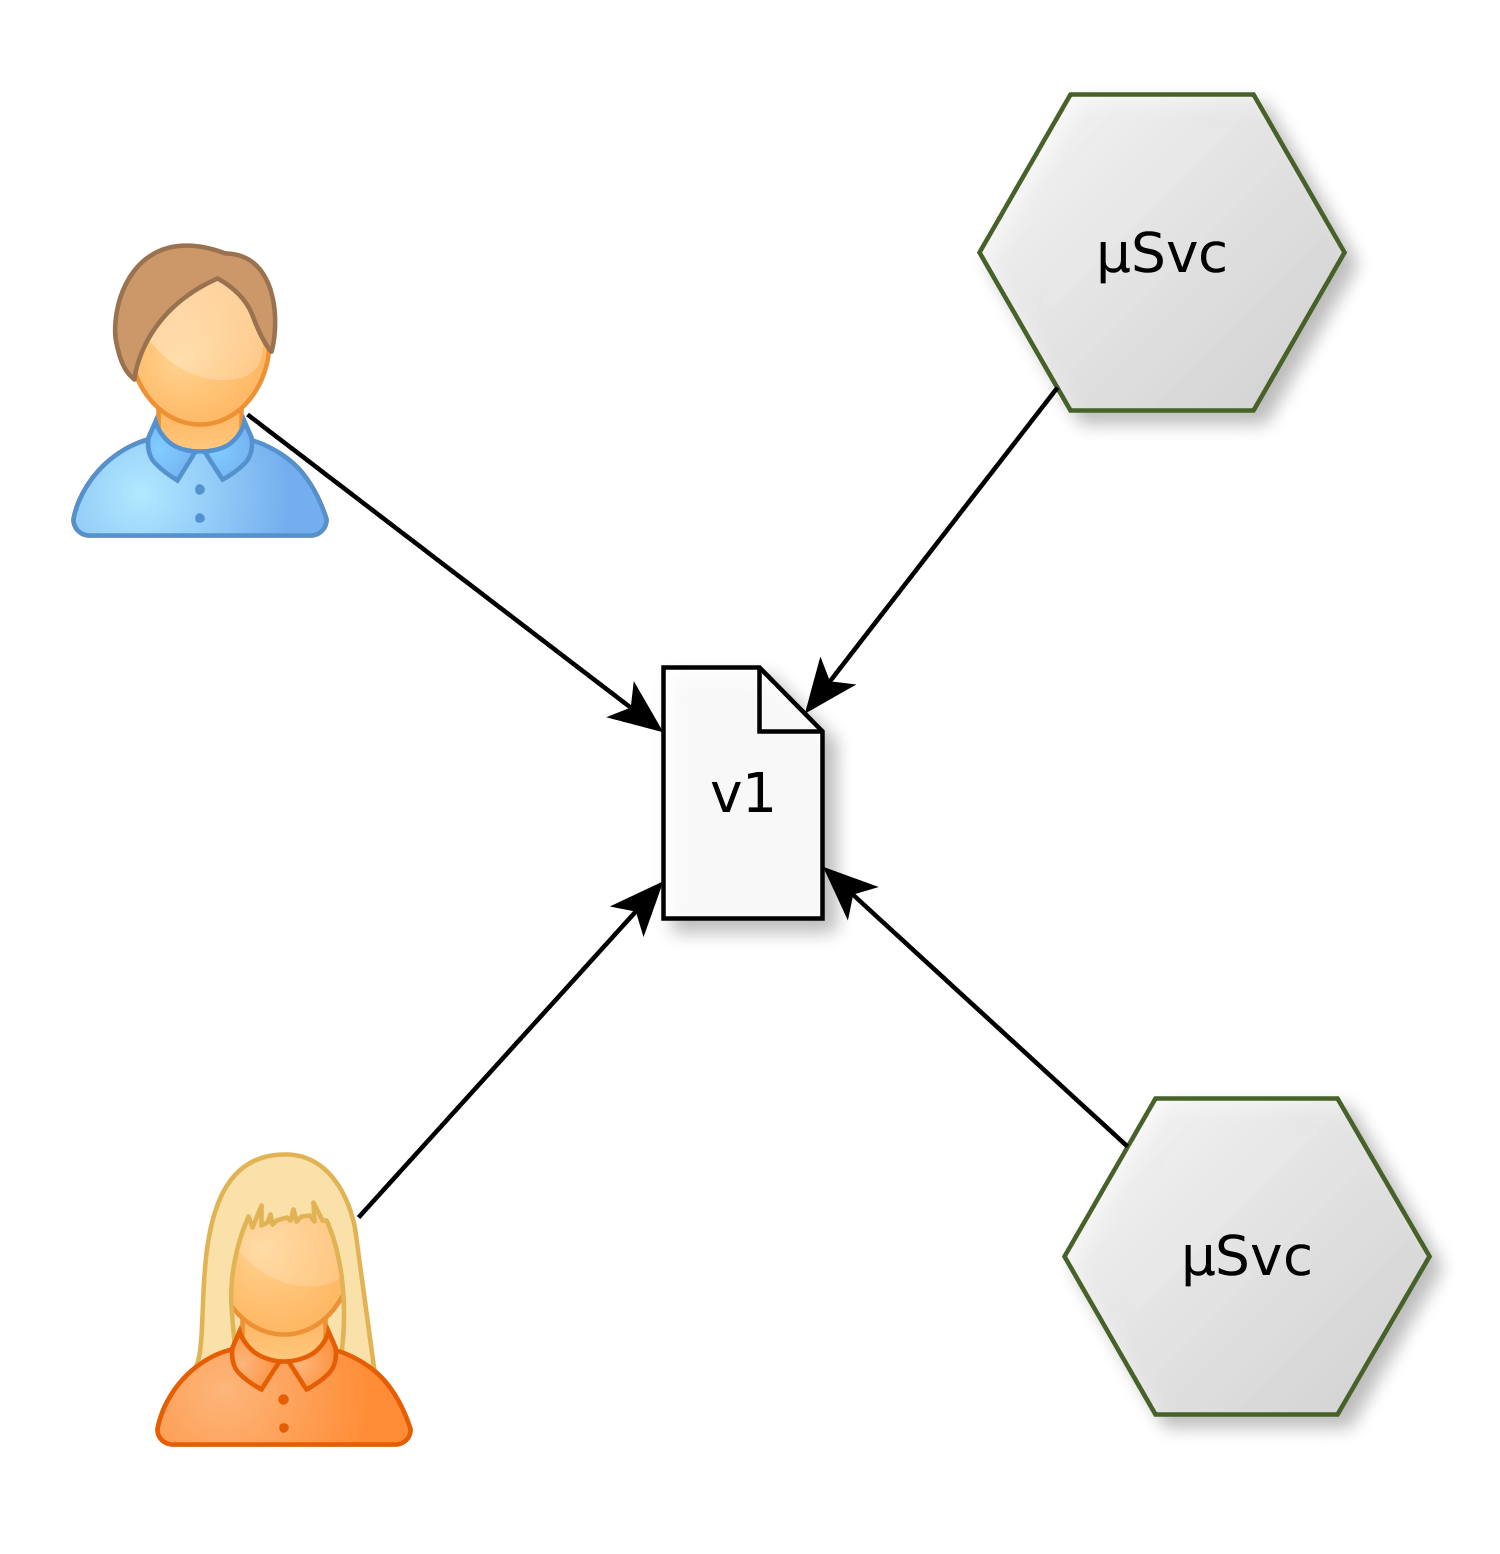
\includegraphics[width=\linewidth]{figures/ACP-initial.png}
%  \caption{initial state}
%  \label{fig:acp-init}
%\endminipage\hfill
%\minipage{0.32\textwidth}
%
%  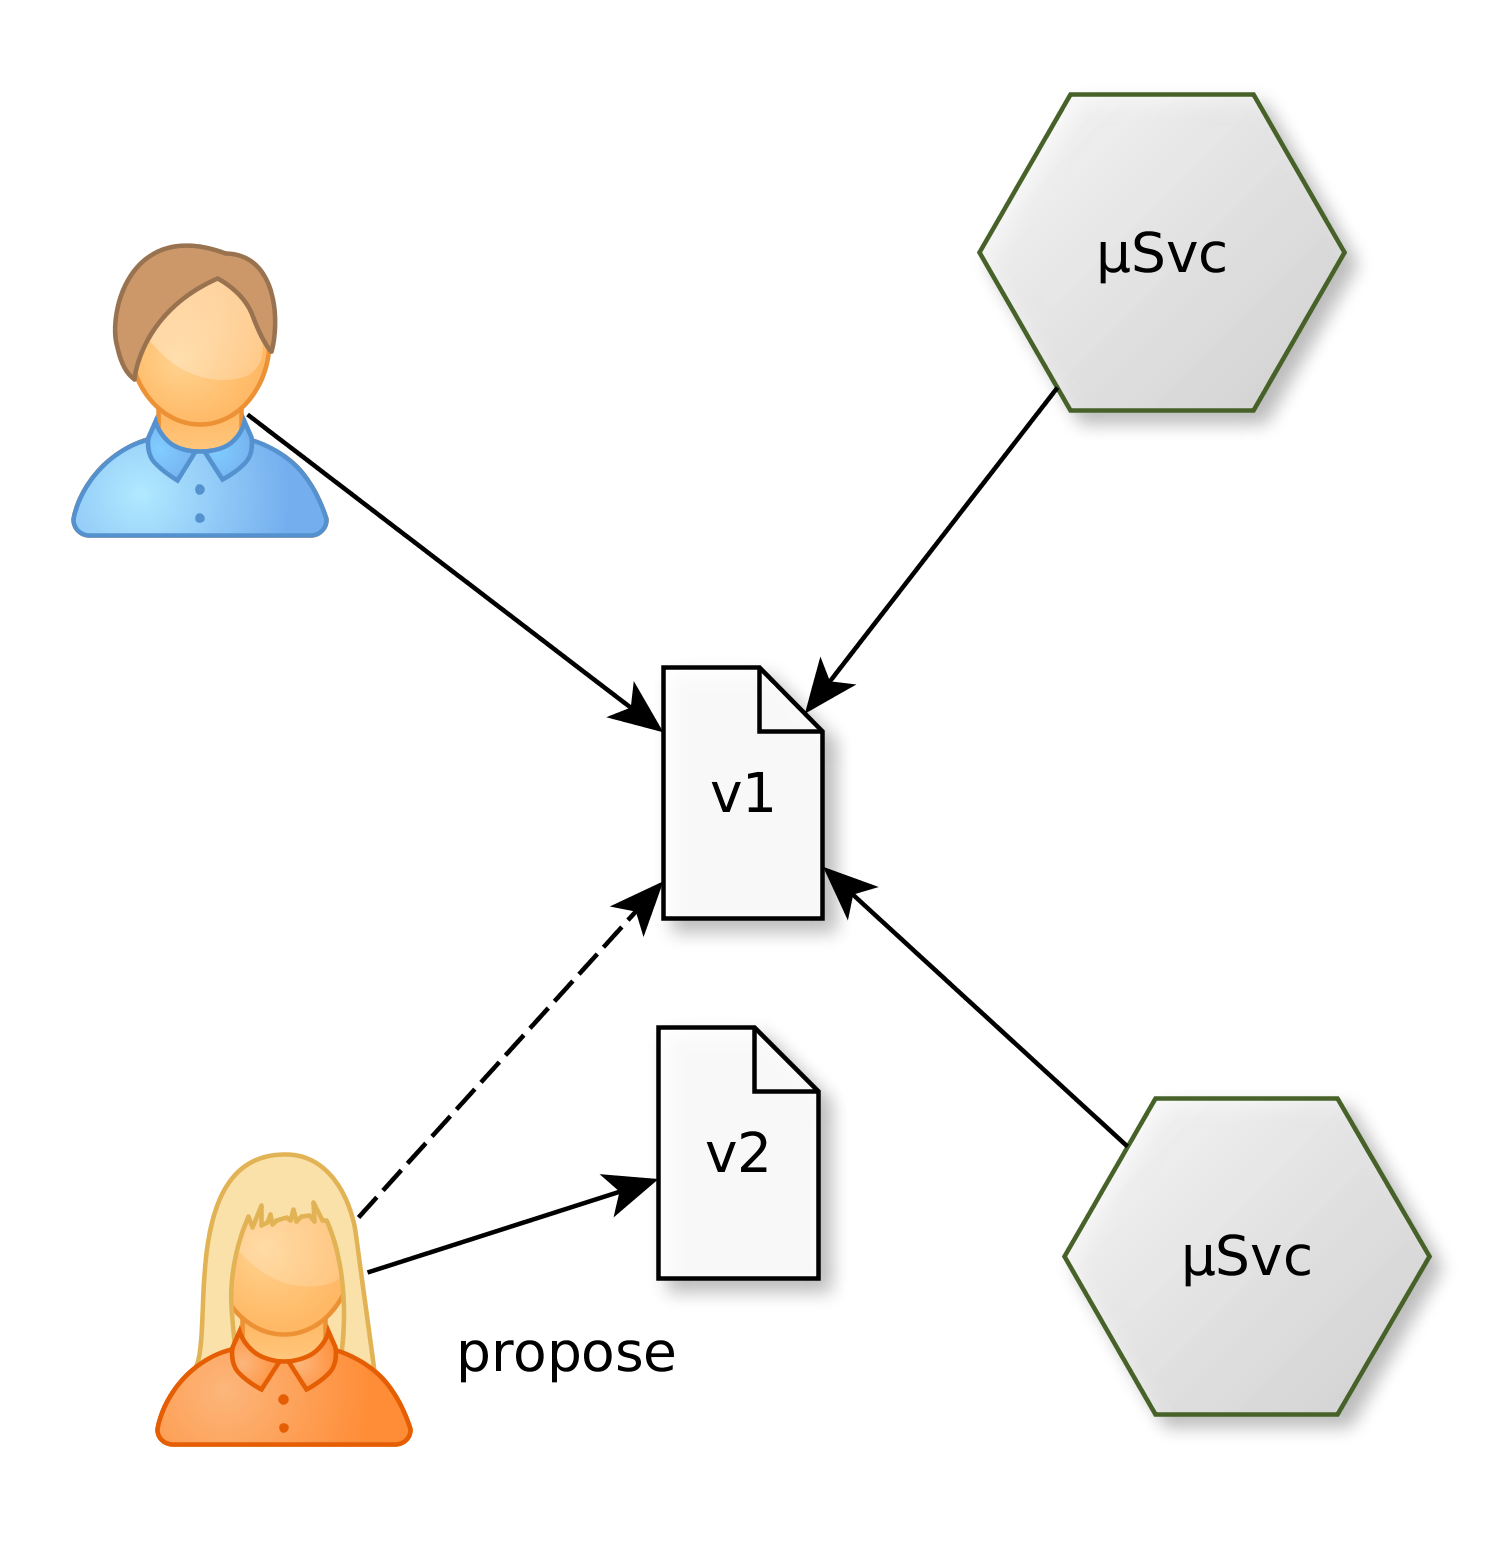
\includegraphics[width=\linewidth]{figures/ACL-propose.png}
%  \caption{state change proposal}
%  \label{fig:acp-propse}
%\endminipage\hfill
%\minipage{0.32\textwidth}
%
%  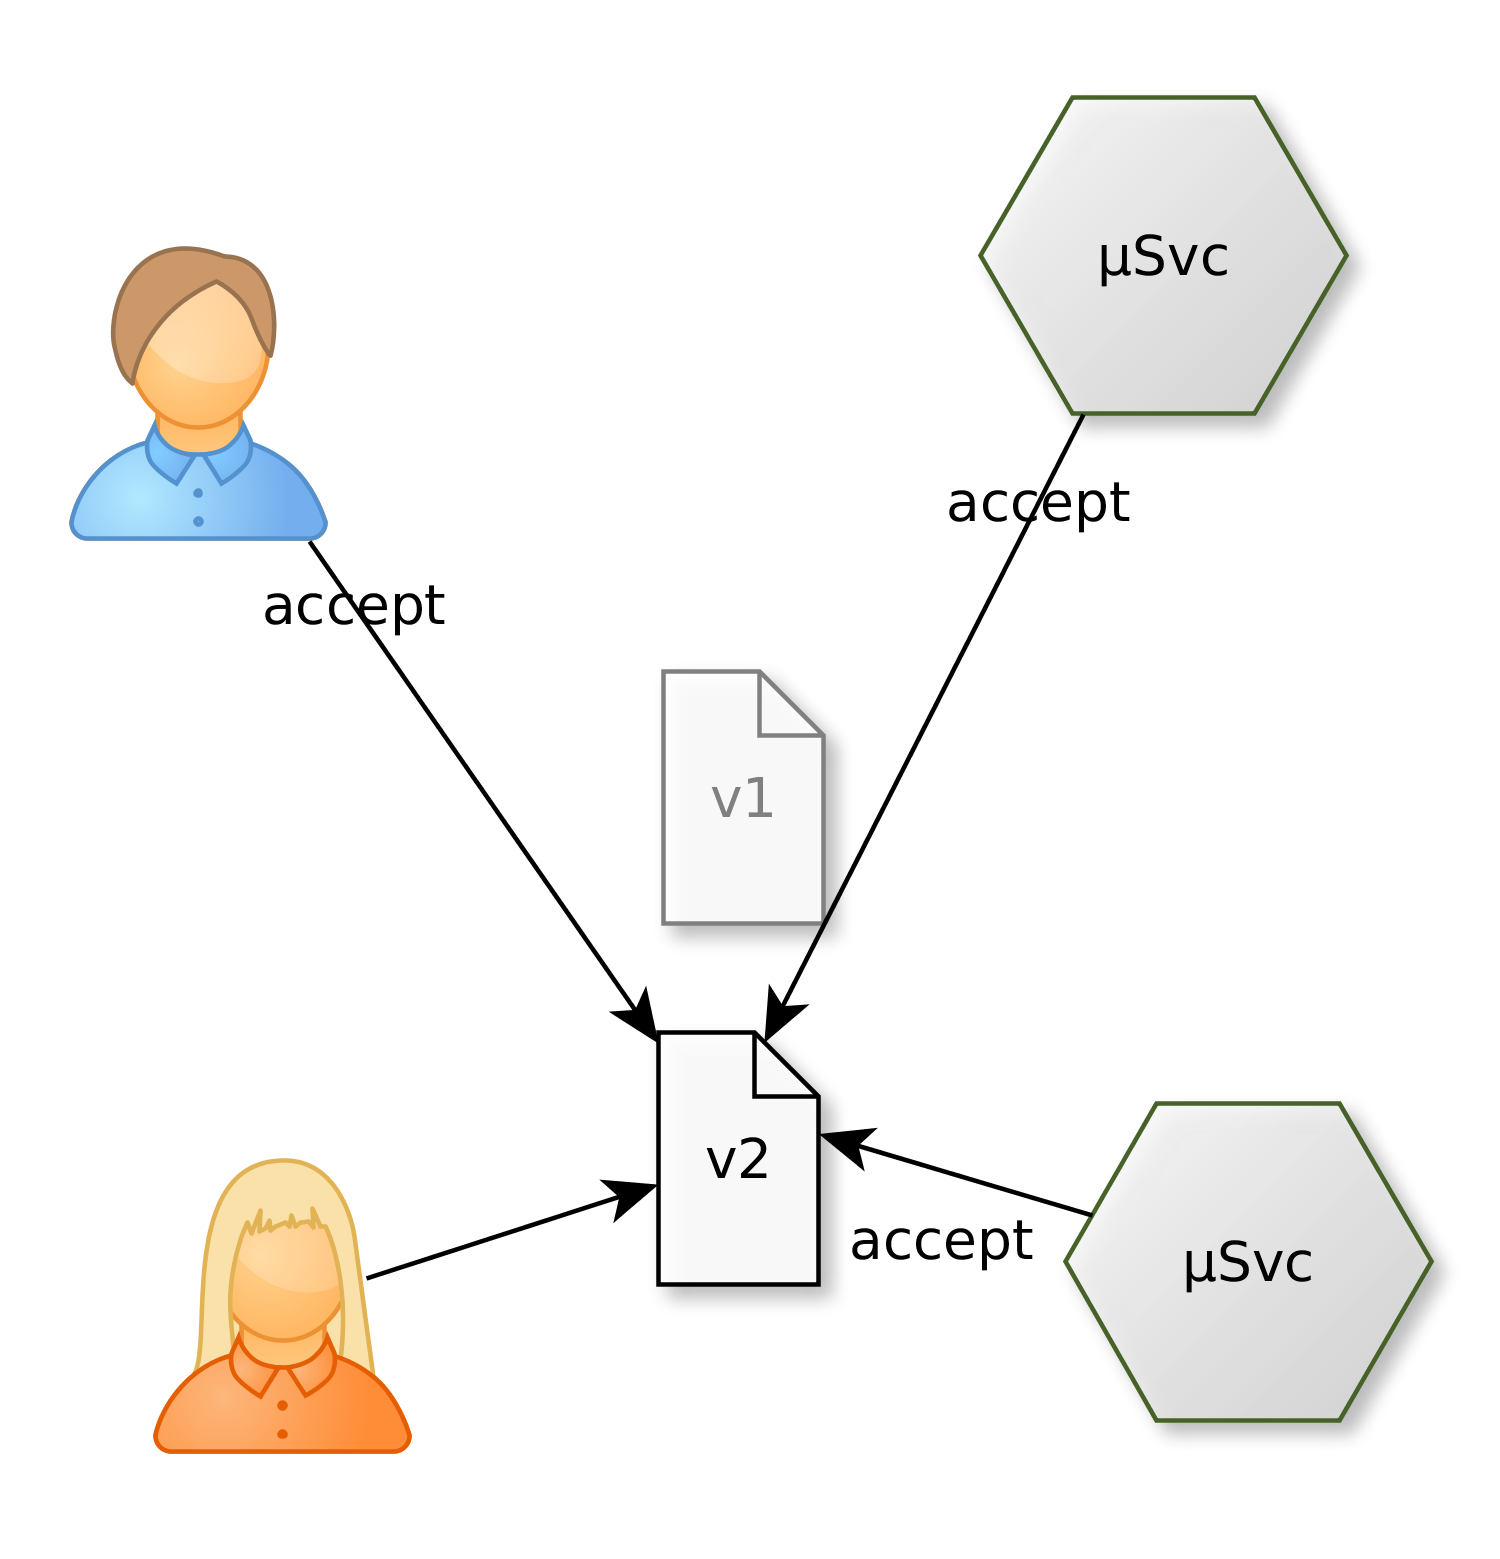
\includegraphics[width=\linewidth]{figures/ACP-accept.png}
%  \caption{accepting new policy}
%  \label{fig:acp-accept}
%\endminipage\hfill
%\end{figure}

When a participant wants to change policy rules, he defines a new version of the ACL and reports a proposal to the network. Each participant can either accept the new version, deny with a user-defined reason or abstain from answering. If no of the participants denies the proposal, the smart contract provides the new ACL list. 

As an alternative, participants could send deltas instead of full versions of the ACL.\\


\subsection{implementation and on-chain/off-chain design}

\begin{figure}[!h]
  \centering
  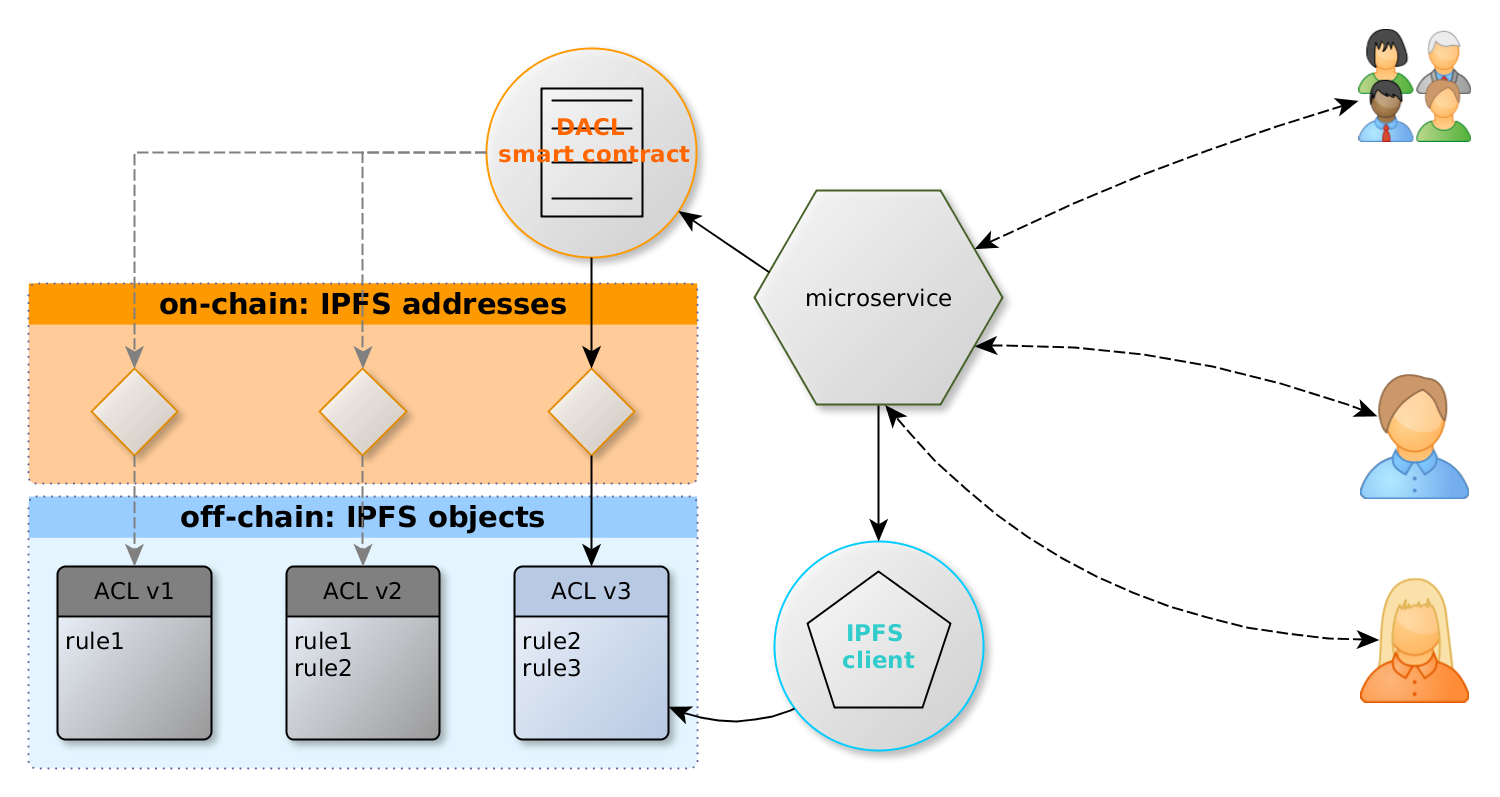
\includegraphics[width=\linewidth]{figures/eth-ipfs-design-without-client.png}
  \caption{DACL architecture}
  \label{fig:ipfs-design-without-client}
  \centering
\end{figure}

After defining that protocol formally, a reference prototype must be implemented using a common language for building microservices. The example will be implemented using NodeJS and Solidity (for developing smart contracts). 

To keep as little as possible data on the blockchain, the smart contract will store IPFS addresses of objects. In the most basic scenario, every microservice implements the policy coordination protocol directly when interacting with IPFS and Ethereum. 

To standardize the coordination, a DACL client can be developed that runs parallel to each microservice and makes the protocol processes available via a well-defined API. It interacts with the smart contract, reads the address from the blockchain and opens the content using an IPFS client.

\newpage

\begin{figure}[!hb]
  \centering
  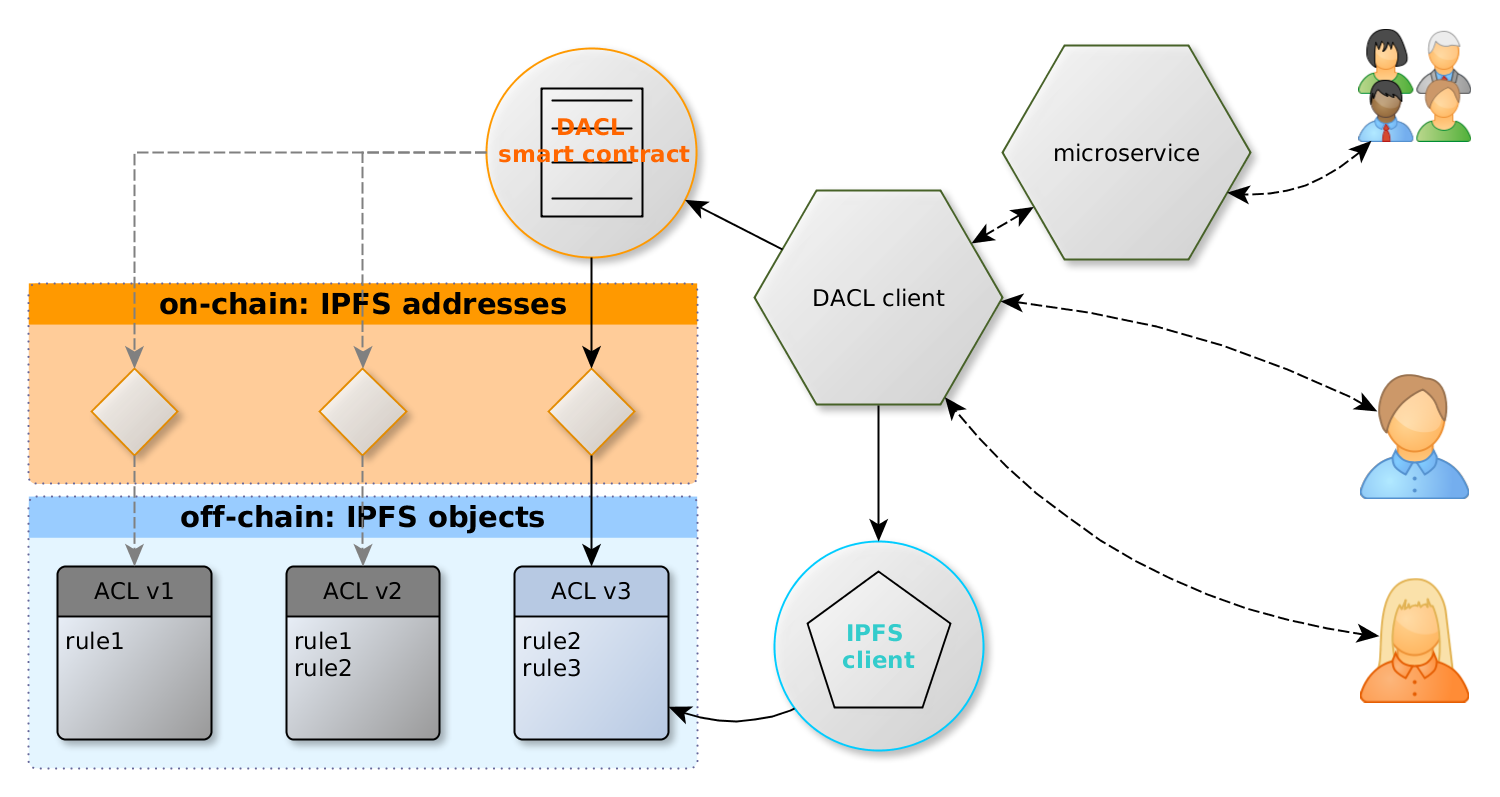
\includegraphics[width=\linewidth]{figures/eth-ipfs-design-with-client.png}
  \caption{DACL architecture with client}
  \label{fig:ipfs-design-with-client}
  \centering
\end{figure}


%
%Each microservice reads and writes a common policy configuration file, which is stored in IPFS and hashed in the Ethereum blockchain. During read, a service must implement own security policies for itself. Interpreting non-owning domain object is optional. For writes (and changes) of that configuration, a service is only able to make a proposal. By using a simple voting system, every service may vote on incoming proposals. Depending on the choice, how consensus is reached, the smart contract finally evaluates pending proposals and in the case of satisfying all conditions, adds the new configuration to the network.



\section{Evaluation}

After designing the protocol and implementing a prototype, it is possible to analyze the result regarding trustlessness and decentralization.

\subsection{Security evaluation}

As trustlessness was defined as the absence of central authorities, the only way of control is the consensus. The voting system offers a strong protection from malicious actions coming from a minority of a network, but several processes take some time, as kicking members or changing policies. So the security evaluation covers the overall security of DACL. In details, it covers how good the privacy promise is satisfied for a patient. In other words: Can a patient trust the platform, which is secured by DACL?
Back to the protection claim, the first tests will be about majority attacks. With the permission to add new members to the network, one party could add a greater amount of voters to the network to manipulate voting decisions during proposals. The attack aims to change a patient's access control policy. 
The next tests will cover ways of performing a minority attacks, as blocking proposals or changing the local values of known policy configurations. Further analysis will try to find exploits, which might be possible during reconciliation if there are some.
Assuming the network identifies a malicious participant, one evaluation will analyze the time of excluding the member from the network.
Another point of interest is how the system performs in use cases, where mandate changes are required. For example, if a patient loses his private keys, but needs access to the data. Furthermore, the patient can grant a doctor to re-grant his permissions to different parties. Considering one of those parties loses control of his keys, the question is how the patient can revoke those permissions, and how fast he can do that.


\subsection{Performance evaluation}

The performance evaluation analyzes, how much the mechanism affects the initial performance of the application. The basic design of DACL is optimized for fast reading operations, at the expense of the time for changes being committed. The access decision protocol assumes, there is a version of the policy configuration ready for analyzing, and defines how to make a decision. Nevertheless, the performance of analyzing this state might deteriorate with a growing amount of data. For this purpose, a test case with an enormous amount of data with corresponding ACLs will be performed. 
In a similar scenario, the next tests will analyze the performance of handling new policy proposals. In details, the eHealth platform owners may decide, that an entry of data is available, as soon its ACLs are available for processing. Here, a simulation will test a high frequency of new proposals and the target attribute is the time of data being available.


%\section{external attack vectors}
%
%There are also attack vectors from the tools used to implement the prototype, like go-ethereum, IPFS but also the consensus finding the concept of a proposal or Ethereum itself. If there are ways of interrupting the smart contracts in general or performing majority attacks in private networks, it will be discussed, which exploit might be applicable to DACL.
%
%Some of the basic properties of the underlying technologies can be exploited as well. If a malicious participant wants to prevent others from interacting with DACL, and it is possible to let others spend ETH to give denies to false proposals, it might be sufficient for the attacker to have more ETH then others.

\newpage

\section{Timeline}

\begin{list}{-}{ }
\item formally design the DACL protocol
\item (possibly) starting implementation of DACL client
\item Building a prototype of a microservice based application, implementing the protocol and using the DACL policies
\item Evaluating the prototype as a proof-of-concept, referring to defined claims and new problems, found during the modeling and/or implementation process
\end{list}


\section*{Related Work}



\begin{list}{-}{}
% \item Decentralized Access Control in Distributed File Systems (MILTCHEV and SMITH)
%\item Trust Mechanism in Distributed Access Control Model of P2P Networks (Wang, Zhu, Jin, Luo)
\item after-the-fact mandate changes (Hyperledger requirement WG)
\item domain-based security in distributed systems (Yialelis)
\item ethereum whitepaper (Buterin)
% \item Hawk - Blockchain Model of Cryptography \& Smart Contracts (Kosba, Miller, Elaine Shi, Wen, Papamanthou)
% \item Consensus and Cooperation in networked multi-agent systems (Olfati-Saber, Fax, Murray)
\item 
\end{list}

More papers and references are pending. 

\bibliographystyle{IEEEtran}
\bibliography{refs}
%\printbibliograpy



\end{document}